% #######################################
% ########### FILL THESE IN #############
% #######################################
\def\mytitle{IMPLEMENTATION OF BOOLEAN LOGIC IN ARDUINO IDE}
\def\mykeywords{}
\def\myauthor{ANIRUDH VS}
\def\contact{anirudhkratos25@gmail.com}
\def\mymodule{}
% #######################################
% #### YOU DON'T NEED TO TOUCH BELOW ####
% #######################################
\documentclass[10pt, a4paper]{article}
\usepackage[a4paper,outer=1.5cm,inner=1.5cm,top=1.75cm,bottom=1.5cm]{geometry}
\twocolumn
\usepackage{graphicx}
\graphicspath{{./images/}}
%colour our links, remove weird boxes
\usepackage[colorlinks=true,urlcolor=blue,linkcolor=black]{hyperref}
%Stop indentation on new paragraphs
\usepackage[parfill]{parskip}
%% Arial-like font
\usepackage{lmodern}
\renewcommand*\familydefault{\sfdefault}
%Napier logo top right
\usepackage{watermark}
%Lorem Ipusm dolor please don't leave any in you final report ;)
\usepackage{circuitikz}
\usetikzlibrary{calc}
\usepackage{tikz}

\usetikzlibrary{shapes, arrows, chains, decorations.markings,intersections,calc}
\usepackage{lipsum}
\usepackage{xcolor}
\usepackage{listings}
%give us the Capital H that we all know and love
\usepackage{float}
%tone down the line spacing after section titles
\usepackage{titlesec}
%Cool maths printing
\usepackage{amsmath}
\usepackage{tabularx}
%PseudoCode
\usepackage{algorithm2e}
\usepackage{pgf}

\usepackage{url}
\usepackage{karnaugh-map}


\titlespacing{\subsection}{0pt}{\parskip}{-3pt}
\titlespacing{\subsubsection}{0pt}{\parskip}{-\parskip}
\titlespacing{\paragraph}{0pt}{\parskip}{\parskip}
\newcommand{\figuremacro}[5]{
    \begin{figure}[#1]
        \centering
        \includegraphics[width=#5\columnwidth]{#2}
        \caption[#3]{\textbf{#3}#4}
        \label{fig:#2}
    \end{figure}
}

\lstset{
frame=single,
breaklines=true,
columns=fullflexible
}

\thiswatermark{\centering \put(-15,-100.0){
\includegraphics[scale=0.3]{logo}} }
\title{\mytitle}
  \author{\myauthor\hspace{1em}\\\contact\\FWC22099    IITH-Future Wireless Communications     Assignment-1\hspace{0.5em}\hspace{0.5em}\mymodule}
\date{}
\hypersetup{pdfauthor=\myauthor,pdftitle=\mytitle,pdfkeywords=\mykeywords}
\sloppy
% #######################################
% ########### START FROM HERE ###########
% #######################################
 
 \begin{document}
 \maketitle
     \tableofcontents
  \textbf{}{\mykeywords}
 \section{Abstract}
 
      The objective of this manual is to show how to obtain the output expression for the karnaugh map shown above :
     
      \begin{center}
      F = X'Y' + YZ
      \end{center}

\section{Introduction}
 
\paragraph{K-map:}
It is a systematic way of simplifying Boolean expressions. With the help of the K-map method, we can find the simplest POS and SOP expression, which is known as the minimum expression. The K-map provides a cookbook for simplification.Just like the truth table, a K-map contains all the possible values of input variables and their corresponding output values. However, in K-map, the values are stored in cells of the array. In each cell, a binary value of each input variable is stored.The K-map method is used for expressions containing 2, 3, 4 variables. Here in the given equation we have 3 inputs. If there are more, we can use more variables.
      
      
      







\section{Components}
       \begin{tabularx}{0.5\textwidth} {
  | >{\centering\arraybackslash}X
  | >{\centering\arraybackslash}X
  | >{\centering\arraybackslash}X | }
\hline
\textbf{Component} &  \textbf{Value} & \textbf{Quantity}\\
\hline
Arduino UNO &  & 1 \\  
\hline
Bread board & - & 1 \\
\hline
Jumper wires & M-M & 8 \\
\hline
Led & - & 1\\
\hline
Resistor & 150ohms & 1\\
\hline




\end{tabularx}

\begin{center}
   
\end{center}
       \subsection{Arduino} \vspace{5mm}
      The Arduino Uno consists of ground pins, some analog input pins from A0 to A3(a0-a3) and digital pins from D1 to D13(d1-d13) which can be used for both input as well as output. It also has two power pins that can generate 3.3V and 5V.In the following exercises, only the ground, 5V and digital pins will be used. here the arduino connection is the most important to run the code and execute it.
   
 
       
\vspace{1cm}
\section{Boolean Equation}
By solving this, we the given following K-map diagram and Boolean equation as follows:
\begin{center}
F = X'Y' + YZ
\end{center}


\section{Truth table for given K-map}
\begin{tabularx}{0.5\textwidth} {
  | >{\centering\arraybackslash}X
  | >{\centering\arraybackslash}X
  | >{\centering\arraybackslash}X
  | >{\centering\arraybackslash}X
  | >{\centering\arraybackslash}X | }
  \hline
 X & Y & Z & A & F\\
\hline
0 & 0 & 0 & 0 & 0 \\  
\hline
0 & 0 & 0 & 1 & 1 \\
\hline
0 & 0 & 1 & 0 & 0 \\
\hline
0 & 0 & 1 & 1 & 1 \\
\hline
0 & 1 & 0 & 0 & 1 \\  
\hline
0 & 1 & 0 & 1 & 1 \\
\hline
0 & 1 & 1 & 0 & 0 \\
\hline
0 & 1 & 1 & 1 & 1 \\
\hline
1 & 0 & 0 & 0 & 0 \\
\hline
1 & 0 & 0 & 1 & 1 \\
\hline
1 & 0 & 1 & 0 & 0 \\
\hline
1 & 0 & 1 & 1 & 1 \\
\hline
1 & 1 & 0 & 0 & 1 \\
\hline
1 & 1 & 0 & 1 & 1 \\
\hline
1 & 1 & 1 & 0 & 0 \\
\hline
1 & 1 & 1 & 1 & 1 \\
\hline
\end{tabularx}
\begin{center}
TABLE 1
\end{center}

\vspace{5cm}

\section{Hardware}
\textbf{1.} Connect Arduino to the computer and upload the code in to the arduino.
\hfill \break
\hfill \break
\textbf{2.} Make 2,3,4 pins in the Arduino as the input pins and 13 pin as the output pin. 
\hfill \break
\hfill \break
\textbf{3.} Corresponding to the given inputs and output lines, It will be obtained at 10 pin.
\hfill \break
\hfill \break
\textbf{4.}. The builtin led in arduino is the indication of the output.




\section{Kmap Diagram from Question}
Given, Solving the Kmap diagram to find the values of substituing in the equation of F. The values of X,Y,Z,X',Y' will be found.

	\begin{karnaugh-map}[4][2][1][$YZ$][$X$]
		\manualterms{1,1,0,1,0,0,0,1}
		\implicant{0}{1}
		\implicant{3}{7}
	\end{karnaugh-map}	
	
(Note:- As per the equation, F=X'Y' + YZ. Here in the kmap diagram let us assume that X = X3X2 and YZ = X1X0. If the value of X=0 then X'=1 and that of the X=1 then X'=0. It same follows for Y also.)


\section{Circuit Diagram for the Obtained Equation}

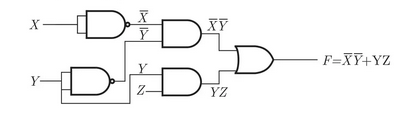
\includegraphics{circuit.png}
 
 
\section{Software}
\textbf{Observe the circuit and verify the program by executing the link provided below.}\\
\begin{center}
\fbox{\parbox{8.5cm}{\url{https://github.com/VSAnirudh2509}}}
\end{center}
\end{document}
